\chapter{Methods}

\section{JESRON MARUDUT HATUAN/1164077}
\subsection{Teori}
Penyelesaian Tugas Harian 5
\begin{enumerate}
\item Random Forest dan Ilustrasi Gambar
\begin{itemize}
\item Pengertian Random Forest:

Random forests merupakan sebuah metode dalam pembelajaran untuk klasifikasi, regresi dan tugas-tugas lain yang telah berperasi dengan membangun banyak pohon keputusan pada saat latihan hingga menciptakan kelas yang merupakan mode kelas atau klasifikasi atau beberapa prediksi dari setiap tree atau pohon.

\item Ilustrasi Gambar Random Forest :
\begin{figure}[ht]
\centering
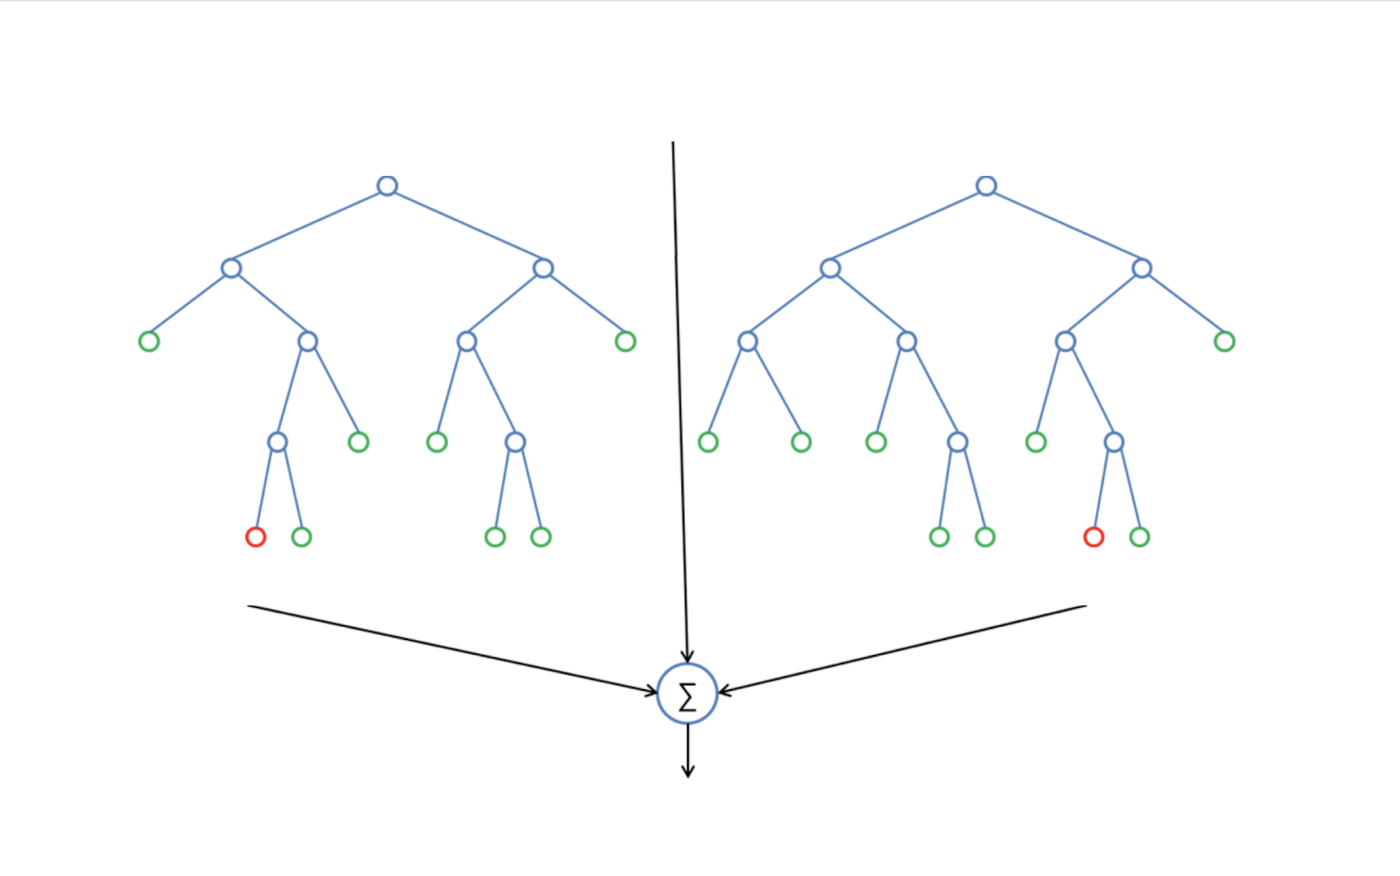
\includegraphics[scale=0.5]{figures/c3jesron1.png}
\caption{Gambar Random Forest}
\label{contoh}
\end{figure}
\end{itemize}
\item Langkah-langkah Membaca Dataset

Berikut adalah langkah-langkah membaca dataset :
\begin{itemize}
\item Pertama-tamma buka applikasi Anaconda Navigator lalu jalankan Syder, kemudian import libraries yang mau dibuat
\item Selanjutnya masukkan kode python untuk membaca file csv, lalu run applikasinya

\begin{figure}[ht]
\centering
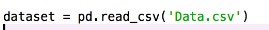
\includegraphics[scale=0.8]{figures/c3jesron2.jpeg}
\caption{Gambar Code Python}
\label{contoh}
\end{figure}

\item Maka pada jendela konsol akan menampilkan pesan berikut:

\begin{figure}[ht]
\centering
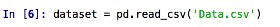
\includegraphics[scale=0.8]{figures/c3jesron3.jpeg}
\caption{Gambar Output}
\label{contoh}
\end{figure}

\item Dan dari jendela explorer akan tampil dataset yang sudah diimport.

\begin{figure}[ht]
\centering
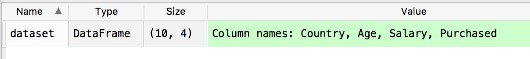
\includegraphics[scale=0.5]{figures/c3jesron4.jpeg}
\caption{Gambar Import Dataset}
\label{contoh}
\end{figure}

\item Selanjutnya klik dataset cell, maka akan muncul seperti berikut :
\item Seperti yang terlihat pada gambar tersebut dataset ini memiliki Kolom Country, Age, dan Salary sebagai kolom

\begin{figure}[ht]
\centering
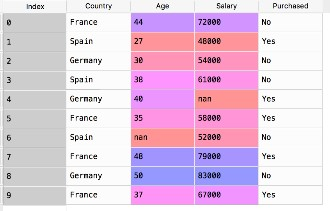
\includegraphics[scale=0.5]{figures/c3jesron5.jpeg}
\caption{Gambar Hasil Dataset Sel}
\label{contoh}
\end{figure}

\item Purchased sebagai dependent variable-nya.
\item Selanjutnya buat 2 matrix of features yang berisi values dari independent variable dan dependent variable.
\item Selanjutnya, masukan perintah berikut :

\begin{figure}[ht]
\centering
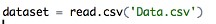
\includegraphics[scale=0.8]{figures/c3jesron6.jpeg}
\caption{Gambar Masukkan Perintah}
\label{contoh}
\end{figure}

\item Perintah yang telah dilakukan gunanya untuk menampilkan dataset.
\item Lalu klick dataset tersebut maka muncul tabel berisi dataset.
\end{itemize}

\item Cross Validation

Cross Validation adalah sebuah teknik untuk memvalidasi model agar dapat menilai bagaimana hasil dari sebuah statistik analisis yang akan menggeneralisasi kumpulan beberapa data independen. Teknik ini lebih sering digunakan untuk melakukan prediksi model dan memperkirakan seberapa akurat sebuah model prediktif ketika sedang dijalankan dalam sebuah praktiknya. Dalam sebuah masalah prediksi, sebuah model biasanya diberikan kumpulan data (dataset) yang telah diketahui untuk digunakan dalam menjalankan pelatihan (dataset pelatihan), serta kumpulan data yang tidak diketahui (atau data yang pertama kali dilihat) terhadap model yang diuji (pengujian dataset)

\item Maksud dari score 44\% pada random forest, 27\% pada decission tree dan 29\%dari SVM.

Maksud dari score 27\% pada decission tree adalah hasil dari  presentasi dari perhitungan dataset, sedangkan maksud dari score 29\% pada SVM adalah dengan pendekatan jaringan saraf. Hasilnya didapat dari valdasi silang untuk memastikan bahwa membagi training test dengan cara yang berbeda. Sehingga outputnya 44\% untuk hutan acak, 27\% untuk pohon keputusan, dan 29\% untuk SVM.

\item Confusion Matrix Dan Ilustrasinya
\begin{enumerate}
\item Perhitungan confusion matrix adalah sebagai berikut, akan saya beri contoh sederhana yaitu pengambilan keputusan untuk mendapatkan bantuan beasiswa. Saya menggunakan dua atribut, yaitu rekening listrik dan gaji. Ini adalah pohon keputusannya:
\begin{figure}[ht]
\centering
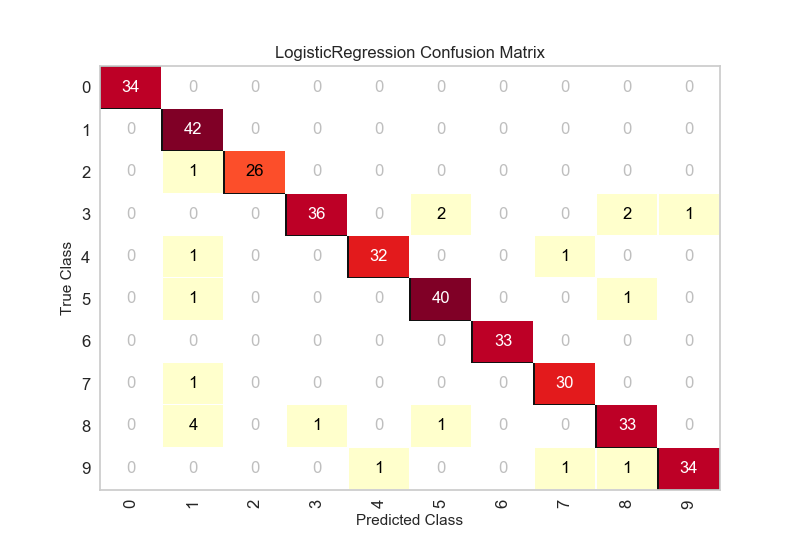
\includegraphics[scale=0.5]{figures/c3jesron7.png}
\caption{Pohon Keputusan}
\label{contoh}
\end{figure}
\end{enumerate}

Selanjutnya data testingnya adalah

\begin{figure}[ht]
\centering
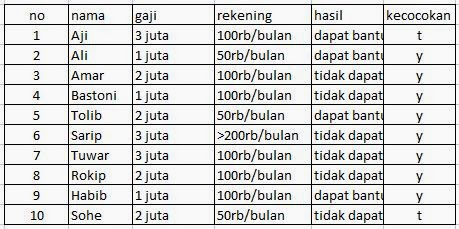
\includegraphics[scale=0.5]{figures/c3jesron8.jpg}
\caption{Gambar Data Testing}
\label{contoh}
\end{figure}

Pertama-pertama, kita lakukan adalah mencari 4 nilai yaitu a,b,c, dan d:

a= 5

b= 1

c= 1

d= 3

Hingga kita dapat mencari nilai Recall, Precision, accuracy dan Error Rate

Recall =3/(1+3) = 0,75

Precision = 3/(1+3) = 0,75

Accuracy =(5+3)/(5+1+1+3) = 0,8

Error Rate =(1+1)/(5+1+1+3) = 0,2

\item Voting Random Forest Dan Ilustrasi Gambarnya.

\begin{itemize}
\item Pengertian Voting pada Random Forest
Voting yaitu suara untuk setiap target yang diprediksi pada saat melakukan Random Forest. Pertimbangkan target prediksi dengan voting tertinggi sebagai prediksi akhir dari algoritma random forest.

\item Gambar Voting Random Forest :
\begin{figure}[ht]
\centering
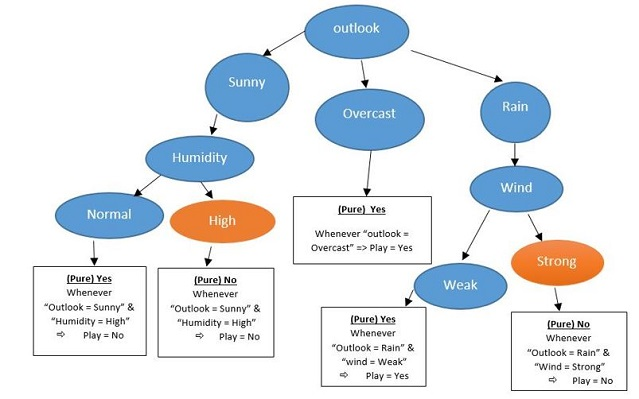
\includegraphics[scale=0.8]{figures/c3jesron9.jpg}
\caption{Gambar Voting Random Forest}
\label{contoh}
\end{figure}
\end{itemize}
\end{enumerate}

\section{The data}
PLease tell where is the data come from, a little brief of company can be put here.

\section {Mhd Zulfikar Akram Nasution / 1164081}
\subsection {Teori}
\begin{enumerate}
\item Random Forest
\par
Ramdom Forest adalah hutan yang acak, dimana maksudnya yaitu terdapat banyak pohon-pohon yang mana disetiap pohon tersebut memiliki atribut yang berbeda-beda, random forest disebut juga kumpulan pohon-pohon keputusan. contoh random forest seperti gambar 3.1
\begin{figure}[ht]
\centering
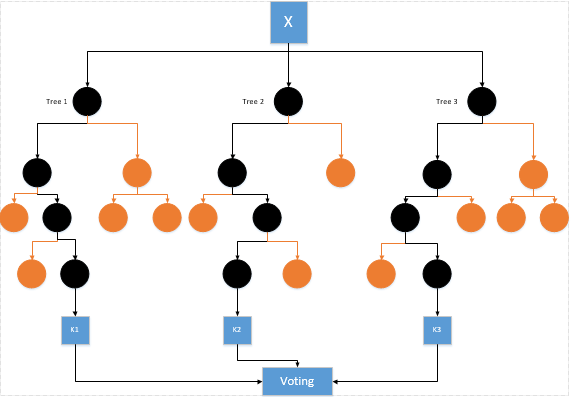
\includegraphics[scale=0.6]{figures/RF/1_1.png}
\caption{Random Forest}
\end{figure}
\item Cara membaca dataset kasus
\begin{itemize}
\item Buka aplikasi spyder untuk membuka dan membaca kodingan dataset
\item Kemudian buat  variable imgatt untuk memasukkan atribut label
\item Lalu uji coba kodingan untuk mengetahui apa hasil dari dataset tersebut
\item imgatt.head() untuk melihat sebagian data awal
\item .shape untuk melihat jumlah data
\item .pivot untuk merubah atribut menjadi kolom
\par
Dengan menguji coba kodingan yang ada pada spyder kita akan dapat membaca dataset yang ada.
\end{itemize}
\item Cross Validation
\par 
Cross Validation adalah sebuah metode statistik yang digunakan untuk mengevaluasi kinerja model, dimana data dipisah menjadi dua subset yaitu data proses pembelajan dan data evaluasi atau validasi.
\item Arti 44 persen pada RF, 27 persen pada Decission Tree, dan 29 persen pada SVM.
\begin{itemize}
\item 44 persen pada Random Forest adalah menjunjukkan hasil yang sempurna pada keputusan yang diambil, biasanya hasil keputusan yang dicapai sekitar 42-44 persen.
\item 27 persen pada Decission Tree adalah menunjukkan hasil keputusan pada tiap-tiap tree dari dataset yang ada.
\item 29 persen pada SVM menunjukkan hasil keputusan dengan klasifikasi dari dataset yang ada.
\end{itemize}
\item Confusion Matrix
\begin{itemize}
\item Pertama import confusion matrixnya
\item Kemudian Plot confusion matrix
\item Lalu sesuaikan plotnya dengan nama data yang ada
\item Setelah itu plot kembali
\end{itemize}
\par
Contoh hasil connfusion matrix pada gambar 3.2
\begin{figure}[ht]
\centering
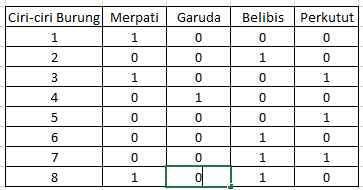
\includegraphics[scale=0.9]{figures/RF/1_2.png}
\caption{Confusion Matrix}
\end{figure}
\item Voting
\par
Voting adalah hasil akhir dari keputusan yang ada pasa setiap pohon di random forest, maksudnya ialah setiap keputusan yang telah dikumpulkan maka akan di voting bahwa hasil tersebut adalah hasil yang benar. Misalnya kita dapat lihat pada gambar 3.3 yaitu dari beberapa ciri-ciri yang ada dapat di voting atau disimpilkan hasil yang paling banyak dimiliki oleh burung belibis, sehingga dapat disimpulkan bahwa dari ciri- tersebut ialah merupakan ciri-ciri dari burung belibis. 
\begin{figure}[ht]
\centering
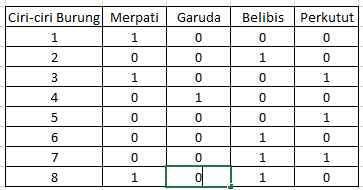
\includegraphics[scale=0.9]{figures/RF/1_2.png}
\caption{Voting}
\end{figure}

\end{enumerate}

\section{Method 1}
Definition, steps, algoritm or equation of method 1 and how to apply into your data
\section{Method 2}
Definition, steps, algoritm or equation of method 2 and how to apply into your data